\begin{spacing}{1}
    \chapter*{Abstract}
\end{spacing}
\begin{wrapfigure}{r}{0.3\textwidth}
    \begin{center}
      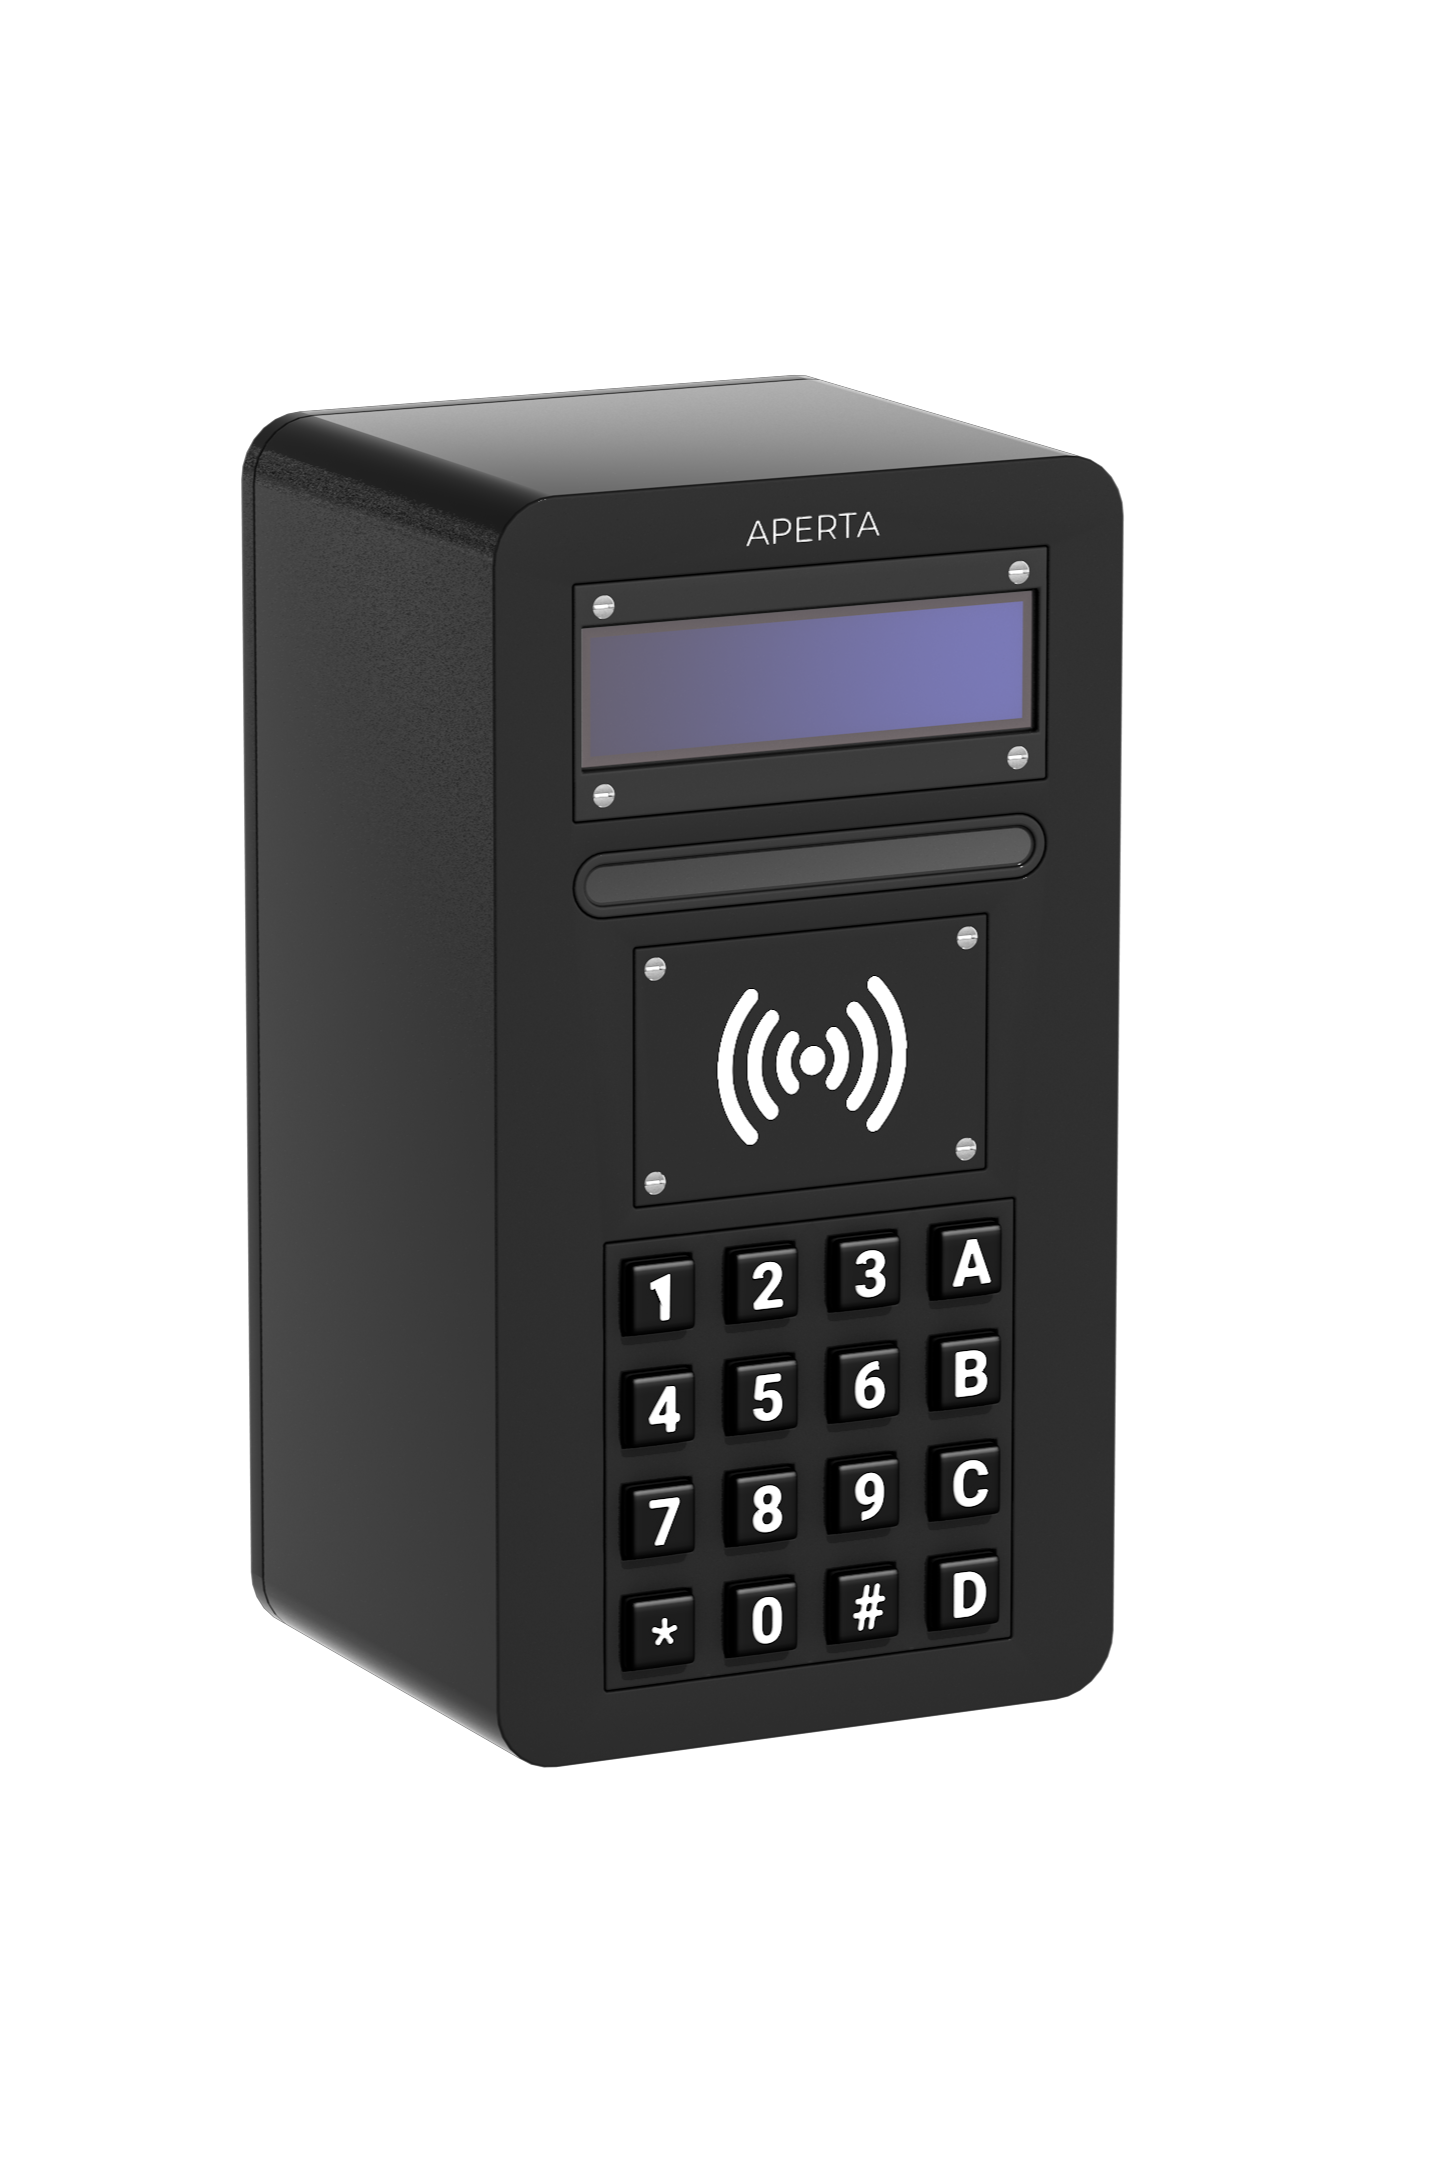
\includegraphics[width=0.5\textwidth]{pics/all-in-package.png}
    \end{center}
\end{wrapfigure}
It is impossible to imagine this world without cars. In Austria alone, more than 5 million cars are registered \cite{StatAustPKW}. According to Statistics Austria, this number has been growing steadily for more than 15 years. In order to be able to guarantee the safety of the occupants, it is recommended to park the vehicle in a garage or a covered area. There, environmental influences such as hail are no longer a major threat.
With the ever-advancing connectivity of the near environment, such as front doors with fingerprint access control or blinds that can be operated with a smartphone, APERTA brings the IOT to the garage.
APERTA is a complete system that can be retrofitted to garages with electric doors. It is possible to open the garage door as usual with the help of a number field or an NFC card. What sets APERTA apart, however, is an integrated license plate recognition system that no longer requires a handheld transmitter or anything similar. The license plate number is entered via the web dashboard, and the door can then recognize it when approached and controls the door opening mechanism.

\newpage
\begin{spacing}{1}
    \chapter*{Zusammenfassung}
\end{spacing}
\begin{wrapfigure}{r}{0.3\textwidth}
    \begin{center}
      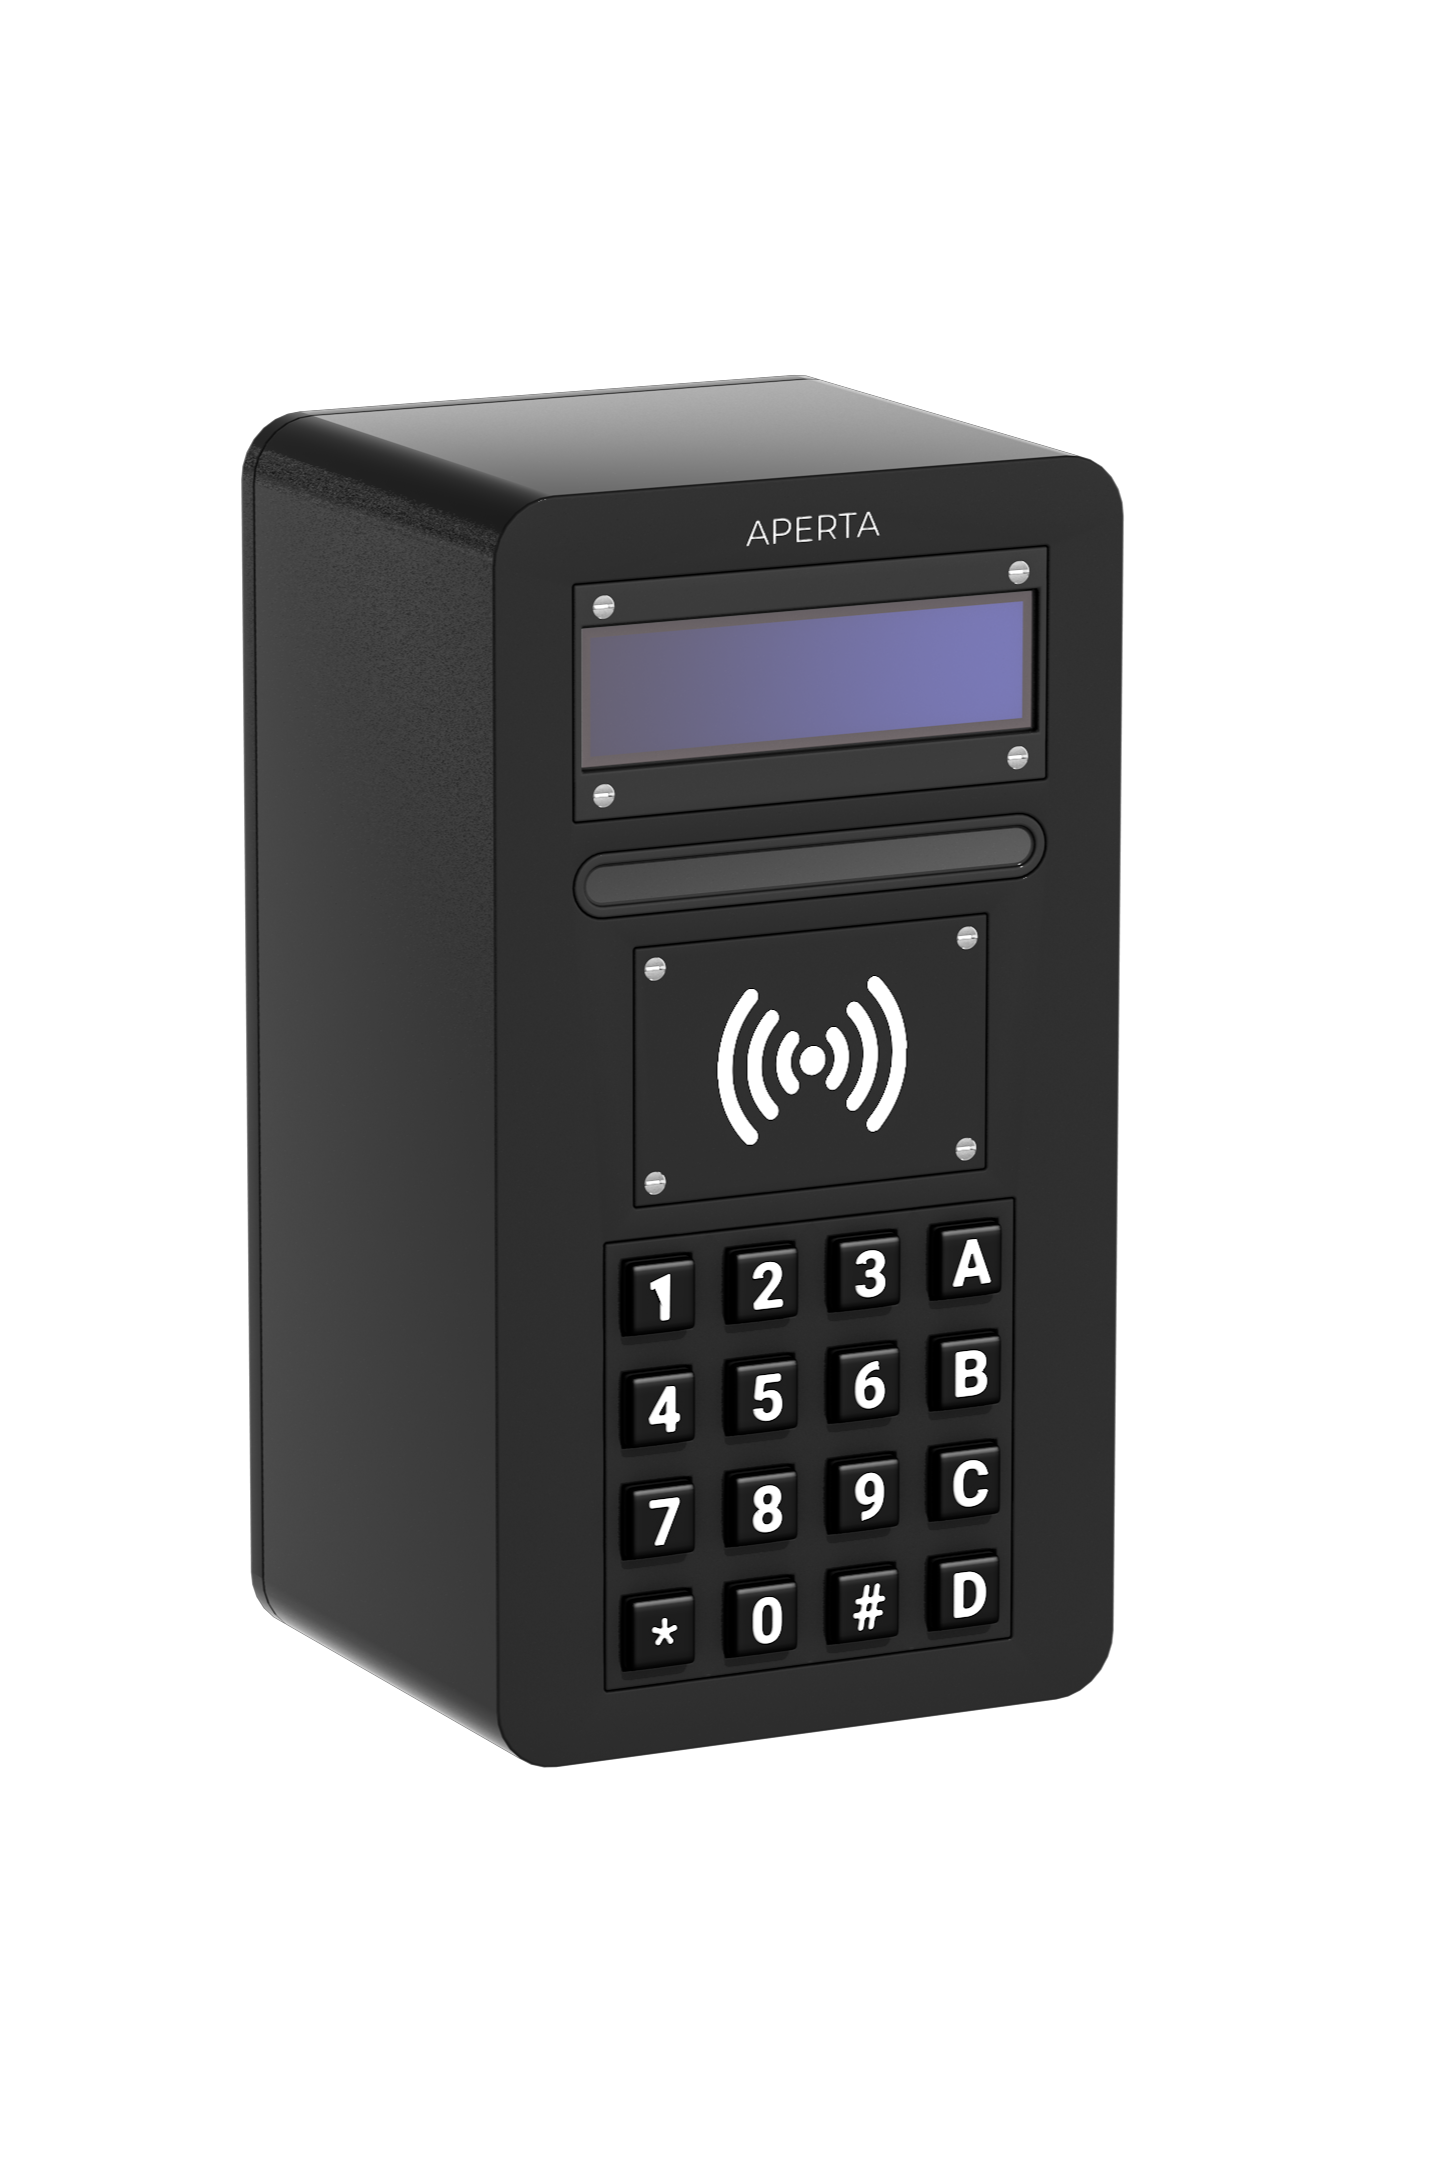
\includegraphics[width=0.5\textwidth]{pics/all-in-package.png}
    \end{center}
\end{wrapfigure}
Autos sind aus dieser Welt nicht mehr wegzudenken. Alleine in Österreich sind mehr als 5 Millionen Personenkraftwagen zugelassen \cite{StatAustPKW}. Dieser Bestand wuchs nach Angaben der Statistik Austria seit mehr als 15 Jahren kontinuierlich an. Um die Sicherheit der Insassen gewährleisten zu können, wird empfohlen, das Fahrzeug in einer Garage oder einem überdachten Gebiet abzustellen. Dort sind Umwelteinflüsse wie Hagel keine große Gefahr mehr.
Mit der immer weiter voranschreitenden Vernetzung der nahen Umwelt, wie Haustüren mit Fingerabruck-Zugangskontrolle oder mit dem Smartphone bedienbaren Jalousien, kommt mit APERTA das IOT in die Garage.
APERTA ist ein Komplettsystem, welches bei Garagen mit elektrischem Tor nachgerüstet werden kann. Es besteht die Möglichkeit, mithilfe eines Nummernfeldes oder einer NFC-Karte das Garagentor wie gewohnt zu öffnen. Was APERTA aber auszeichnet ist eine integrierte Kennzeichenerkennung, bei der man keinen Handsender oder ähnliches mehr benötigt. Das Kennzeichen wird über das Web-Dashboard eingegeben, und das Tor kann dann bei Annäherung an das Tor dieses erkennen und steuert den Toröffnungsmechanismus an.

